\chapter{Notions liés ou projet}

\section{PGQL}
PGQL est un DSL (Domain Specific Language) pour l'interrogation de modèles de données de graphes de propriétés. Sa syntaxe est basée sur SQL, il vous permet de spécifier des patterns de graphes de haut niveau qui sont appliqués aux sommets et aux arêtes d'un graphe. PGQL prend en charge le regroupement (GROUP BY), l'agrégation (par exemple MIN, MAX, AVG, SUM), le tri (ORDER BY) et de nombreux autres concepts familiers en SQL. De plus, PGQL dispose de puissantes formes d'expression régulière pour l'accessibilité des graphes (fermeture transitive), la recherche du chemin le plus court et du chemin le moins cher.\\
\textbf{Syntaxe :}
\begin{figure}[H]  
  \centering
    
\includegraphics[width=1\textwidth]{annexe/Figures/PGQL_syntaxe1.png}
\end{figure}

Plus précisément, la syntaze de PGQL peut s'écrire comme suit:
\begin{figure}[H]  
  \centering
    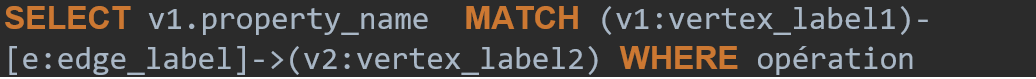
\includegraphics[width=1\textwidth]{annexe/Figures/PGQL_syntaxe2.png}
\end{figure}

\begin{itemize}[label=\textbullet]
\item \textbf{SELECT :} Après ce mot-clé, nous spécifions ce que nous voulons obtenir comme retour de l'exécution de la requête ; dans ce cas, une propriété du sommet \textbf{v1}.
\item \textbf{MATCH :} Après ce mot-clé, nous spécifions le pattern regex, ou quels sommets/arêtes doivent être inclus dans le traitement de la requête.
\item \textbf{WHERE } (optionnel) \textbf{ :} Après ce mot-clé, nous spécifions ce que nous voulons faire avec les données extraites du modèle.
\item \textbf{v1},  \textbf{v2}, et  \textbf{e :} Ce sont des noms optionnels pour les sommets/arêtes que nous traversons ; ils permettent la possibilité d'utiliser cette arête/sommet dans d'autres opérations de la même requête, par exemple si \textbf{v1} n'était pas spécifiée dans la requête je ne pouvais pas obtenir sa propriété dans l'instruction select.
\item \textbf{vertex/edge label (étiquette) :} Elles spécifient exactement les sommets/arêtes que nous voulons inclure dans la requête, elles sont facultatives, et si elles ne sont pas spécifiées, nous obtiendrons tous les sommets/arêtes suivant le pattern que nous avons spécifié, quel que soit leur type.
\item \textbf{Operation :} Ce peut être n'importe quel opération valide, tel que des filtres des agrégations ...etc.
\end{itemize}

\section{Frames et Result-set}
\begin{itemize}[label=\textbullet]
\item Un \textbf{frame} dans PGX est une structure de données, qui est utilisée pour stocker les résultats intermédiaires de notre requête, vous pouvez le considérer comme un tableau contenant les colonnes que nous avons sélectionnées.
\item A \textbf{result-set} en PGX est aussi un frame mais il stocke le résultat final qui doit être communiqué à l'utilisateur une fois que toutes les opérations de la requête sont terminées. C'est un concept similaire à l'objet ResultSet dans JAVA.
\end{itemize}

Exemple d’un Result-set en utilisant le client PGX JShell:\\
\begin{figure}[H]  
  \centering
    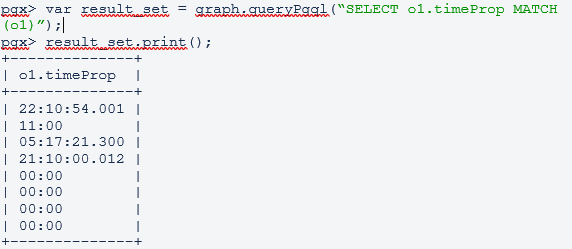
\includegraphics[width=1\textwidth]{annexe/Figures/ResultSet.PNG}
\end{figure}

\section{Architecture PGX.D}
Dans PGX l'utilisateur peut interagir avec le système en utilisant plusieurs types de clients:
\begin{figure}[H]  
  \centering
    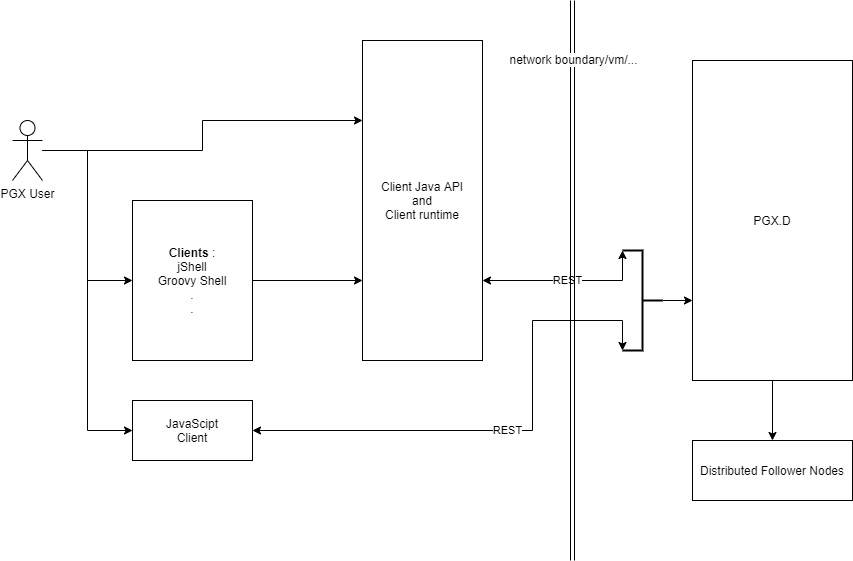
\includegraphics[width=1\textwidth]{annexe/Figures/PGX-Architecture.png}
\end{figure}

\begin{itemize}[label=\textbullet]
\item En exposant l'API Java directement à l'utilisateur via le shell (e.g. Groovy shell, jShell).
\item Utilisation d'un Java-API wrapper et d'une implémentation personnalisée dans la langue hôte (e.g. R and python)
\item Le client JavaScript, qui communique directement avec la webapp au lieu d'utiliser l'API Java.
\end{itemize}

L’\textbf{API Java} expose les fonctionnalités de PGX à l'utilisateur, et elle est responsable de la traduction des requêtes vers REST.\\
Le L’\textbf{In-memory engine}(PGX.D) est responsable du traitement de la requête. Il contient les fonctionnalités suivantes :
\begin{itemize}[label=\textbullet]
\item Charger les graphes de diverses sources de stockage persistant dans la mémoire.
\item Stocker les graphes de la mémoire dans le stockage persistant.
\item Exécuter des algorithmes de graphes sur les graphes en mémoire.
\item Exécuter les requêtes PGQL sur les graphes en mémoire.
\end{itemize}

\section{LDBC benchmark}
Le Social Network Benchmark de l’organisation LDBC (LDBC SNB) est une initiative industrielle et universitaire, formée par les principaux acteurs dans le domaine de la gestion des données sous forme de graphes. Son objectif est de définir un cadre dans lequel différentes technologies basées sur des graphes peuvent être testées et comparées de manière objective, qui peut conduire à l'identification des points de blocage des systèmes et des fonctionnalités requises, et qui peut aider les chercheurs à ouvrir de nouvelles frontières dans les systèmes de traitement des données de type graph à haute performance.


\section{Ghost nodes}
Les « Ghost nodes » ou les sommets fantômes, sont des sommets qui existe sur plusieurs machines à la fois, mais juste l’un de ces sommets est réel.\\
Le sommet réel est stocké dans machine que comporte les propriétés du sommet, les sommet fantômes ne stocke qu’une référence vers le sommet réel pour pouvoir récupérer des données ou cas où le calcule en demande. La figure 28 montre un graphe distribuée sur deux machines ou on utilise des sommets fantômes.\\
Cette technique permet ainsi de faire des calcules localement sans avoir à dupliquer les données sur tous les machines et réduit la communication si non nécessaire.
\begin{figure}[H]  
  \centering
    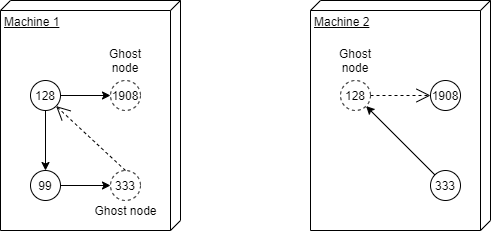
\includegraphics[width=1\textwidth]{annexe/Figures/GhostNodes.png}
  \caption{Exemple d'utilisation des sommets fantômes}
\end{figure}
